% Copyright (C)  2015  Alexander Jankowski, Philipp Hacker.
% Permission is granted to copy, distribute and/or modify this document
% under the terms of the GNU Free Documentation License, Version 1.3
% or any later version published by the Free Software Foundation;
% with no Invariant Sections, no Front-Cover Texts, and no Back-Cover Texts.
% The lincense itself can be found at <https://www.gnu.org/licenses/fdl-1.3>.

\documentclass[numbers=noenddot,a4paper,notitlepage,twoside,BCOR15mm]{scrartcl}
%\documentclass[numbers=noenddot,12pt,a4paper]{scrartcl}

\usepackage{ifoddpage}
\usepackage[infoshow]{tabularx}
\usepackage{fancyhdr}
\usepackage[greek,ngerman]{babel}
\usepackage[T1]{fontenc}
\usepackage[utf8]{inputenc}
\usepackage{libertine}
\usepackage{ziffer}
\usepackage{graphicx}
\usepackage{units}
\usepackage[infoshow]{tabularx}
\usepackage[all]{xy}
\usepackage{amsmath}
\usepackage{amssymb}
\usepackage{wrapfig}
\usepackage{upgreek}
\usepackage{esint}
\usepackage{float}
\usepackage[font=small,labelfont=bf]{caption}
\usepackage{subcaption}
\usepackage{lscape}
\usepackage[backref=page]{hyperref}
\usepackage{cleveref}
\usepackage{csquotes}

\renewcommand{\headrulewidth}{0.1pt}
\renewcommand{\footrulewidth}{0.1pt}
\newcommand{\name}{\text{Philipp Hacker}} %TODO Name des Protokollanten eintragen

\renewcaptionname{ngerman}{\figurename}{Abb. }
\renewcaptionname{ngerman}{\tablename}{Tab.}

\setlength{\parindent}{0pt}

\newcommand{\nummat}[1]{\left[\text{#1}\right]}
\newcommand{\num}[1]{$\left[\text{#1}\right]$}
\newcommand{\degree}{^\circ}
\newcommand{\diff}{\textnormal{d}}
\newcommand{\tenpo}[1]{ 10^{#1}}
\newcommand{\greek}[1]{\greektext#1\latintext}
\newcommand{\ix}[1]{_\text{#1}}
\newcommand{\imag}{\mathbf{i}}
\newcommand{\tilt}[1]{\textit{#1}}
\newcommand{\grad}[1]{\textit{grad}\left(#1\right)}
\newcommand{\divergenz}[1]{\textit{div}\left(#1\right)}
\newcommand{\euler}{\mathnormal{e}}
\newcommand{\fett}[1]{\textbf{#1}}
\newcommand{\einnup}{\hspace{0.2cm}}
\newcommand{\einnum}{\hspace{-0.2cm}}
\newcommand{\zentriert}[1]{\begin{center}#1\end{center}}

\title{Protokoll: Kernspinresonanz -Spektroskopie\\ (Nuclear Magnetic Resonance)} %TODO Name des Versuchs eintragen
\author{Alexander Jankowski, Philipp Hacker}
\date{\today}
\pagestyle{fancy}
\fancyhead[C]{\thepage}
\fancyhead[R]{\name}
\fancyfoot[C]{\thepage}
\fancyhead[L]{Abschnitt \thesection}

\begin{document}
	\maketitle
	\begin{center}
		Betreuer: Carsten Killer\\ %TODO Name des Betreuers eintragen
		Versuchsdatum: 20.11.2015\\ %TODO Datum des Versuchs eintragen
		\begin{table}[h]
			\centering
			Note: %TODO Gute Note erhalten :)
			\begin{tabularx}{1.5cm}{|X|}
				\hline \\ \\
				\hline
			\end{tabularx}
		\end{table}
	\end{center}
	\vspace*{\fill}
	\tableofcontents
	\vfill
	\clearpage
	\section{Motivation}

		Die bildgebende Magnetresonanztomografie ist eines der wichtigsten und fortschrittlichsten medizinischen Verfahren zur nicht-invasiven Untersuchung des menschlichen Körpers. Die physikalische Grundlage dahinter geht auf die Entdeckung von Spin-Echos im Antwortspektrum einer Probe in einem externen, modulierten Magnetfeld durch E. L. Hahn \cite{SpinEcho} zurück. In diesem Versuch sollen einmal die wichtigsten Verfahren zur Kernspin-Resonanz-Spektroskopie nachvollzogen und selbst angewendet werden.

	\clearpage
	\section{Physikalische Grundlagen}

		\subsection{Kernspin in einem externen  Magnetfeld}

				\begin{wrapfigure}{r}{0.3\textwidth}
					\centering
					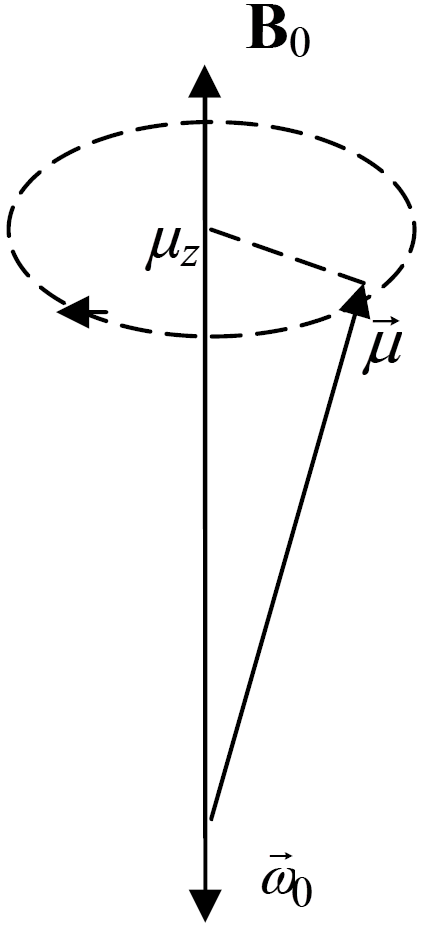
\includegraphics[width=0.25\textwidth]{praezess.png}
					\caption{Präzession eine magnetischen Momentes $\vec{\mu}$ in einem externen Feld $\vec{B}\ix{0}$. \cite{EMAUGreifswaldNMR}}
				\end{wrapfigure}

			Der Spin ist eine rein quantenmechanische Größe von Elementarteilchen. Im klassischen Sinne lässt sich dieser als der Eigendrehimpuls um den eigenen Schwerpunkt mit Variabler Drehachse aber fester Frequenz veranschaulichen, wobei dies nicht als Analogen zu den Formulierungen aus der Quantenphysik verstanden werden kann. Ebenso wie der Gesamtspin der Elektronenhülle $\vec{S}$, mit Quantenzahl $\hbar s\ix{z}=(\vec{S})\ix{z}$ und dessen Betragsquadrat (e.g. Energieaufspaltung) $\vec{S}^2=\hbar^2 S(S+2)$, kann eine analoge Größe für das System der Nuklei im Atomkern definiert werden. Dieser Kern-Gesamtspin $\vec{I}$ erfüllt alle Eigenschaften eines Operators, welcher Drehung ausführt/symbolisiert - damit sind die verschiedenen Kommutatoren, Eigenwertgleichungen und quantenmechanischen Regeln gemeint.\\
			Die unterschiedlichen Arten der ug-,gu-,uu-Kerne - Zahl der Neutronen und Protonen -  können ganz- oder halbzahligen Gesamtspin haben. Kerne mit geraden $n$- und $p$-Zahlen haben auf Grund der anti-parallelen Anordnung $\vec{I}^2 =0\,$. Die Multiplizität des Spin-Zustandes eines Kerns kann mit Hilfe der z-Komponente $I\ix{z}=m\ix{I}\hbar$ - wegen der nicht gleichzeitig messbaren Komponenten beliebig festgelegt - zu $2I+1$ ermittelt werden. Für das in diesem Versuch betrachtete Wasserstoff-Atom kann die magnetischen Spinquantenzahlen $m\ix{I}=\pm 1/2$ haben.\\
			Eine rotierende/gyrierende Ladung besitzt ein magnetisches Moment. Für den Kern gilt \autoref{eq:magnet} mit dem gyromagnetischen Verhältnis $\gamma$, dem Kernmagneton $\mu\ix{K}$ und dem Kern-\tilt{Landé}-Faktor $g\ix{I}$.

				\begin{align}
					\vec{\mu}=\gamma\hbar\vec{I}=g\ix{I}\mu\ix{K}\vec{I} \label{eq:magnet}
				\end{align}

			Ein äußeres Magnetfeld richtet diese magnetische Moment entlang seiner Feldlinien aus. Daraus folgt eine zusätzliche potentielle Energie des Teilchens $V\ix{mag}$ in diesem Feld. Sei o.B.d.A. das homogene, stationäre Magnetfeld in (der) z-Richtung $\vec{B\i}\ix{0}$ zusammen mit dem Spin des Kerns, so ergibt sich \autoref{eq:pot}. Die resultierende \tilt{Zeemanaufspaltung} der Energieniveaus kann bspw. durch ein Photon mit der Frequenz $\omega\ix{0}$ aufgebracht werden. Die Resonanz des Kernspins in externen Feldern liegt demnach genau bei diesem $\omega\ix{0}$.

				\begin{align}
					V\ix{mag}=-\vec{\mu}\vec{B}\ix{0}&=-g\ix{I}\mu\ix{K}\hbar m\ix{I}B\ix{0} \label{eq:pot} \\
					\omega\ix{0}&=\gamma B\ix{0} \label{eq:resonanz}
				\end{align}

			Da nun bekannt ist, dass die Spin-Niveaus nicht zusammenfallen, sondern aufspalten, kann im thermischen Gleichgewicht eine \tilt{boltzmannartige} Verteilung des Besetzungsverhältnisses von \tilt{spin-up} und \tilt{spin-down} mit \autoref{eq:boltz} angeführt werden. Dabei ist die niederenergetische Besetzung \underline{immer} größer als die des höheren Niveaus.\\
			Die kollektive Ausrichtung der Spins im Magnetfeld erzeugt die Magnetisierung $M\ix{z}$. Da das "`\tilt{umdrehen}"' der einzelnen Spin-Richtungen - explizit die Drehachsen - im Magnetfeld einem statischen Prozess gleicht, gilt \autoref{eq:magnetumkl} für die Magnetisierung zum Zeitpunkt $t$. Darin steht $T\ix{1}$ für die sog. \fett{Spin-Gitter-Relaxationszeit}: nach dieser Zeit ist die anfänglich beliebige Spin-Anordnung im Magnetfeld auf das $(1-1/\euler)$-fache der Gleichgewichtsmagnetisierung $M\ix{0}$ angestiegen.

				\begin{align}
					\frac{N_{\uparrow}}{N_{\downarrow}}& =\exp\left(\frac{\hbar\omega\ix{0}}{k\ix{B}T}\right) \label{eq:boltz}\\
					\frac{\diff M\ix{z}}{\diff t}=\frac{M\ix{0}-M\ix{z}}{T\ix{1}}&=\frac{(N_{\uparrow}+N_{\downarrow})\frac{\mu^2B\ix{0}}{k\ix{B}T}-(N_{\uparrow}-N_{\downarrow})\mu}{T\ix{1}} \label{eq:magnetumkl}
				\end{align}

			Der Differentialgleichung \autoref{eq:magnetumkl} genügt die Funktion aus \autoref{eq:magnetfkt} der Magnetisierung in einem externen, homogenen und stationären Magnetfeld zu einer Zeit t nach dem Einschalten. Insbesondere ist zu beachten, das die rein "`thermische"' Magnetisierung in Magnetfeld-Richtung ohne äußeres Feld $M\ix{0}$ entspricht. In x- bzw. y-Richtung verschwindet diese hingegen.

				\begin{align}
					M\ix{z}(t)=M\ix{0}+(M\ix{z}(t=0)-M\ix{0})\exp\left(-\frac{t}{T\ix{1}}\right) \label{eq:magnetfkt}
				\end{align}

				Äquivalent kann man ähnlich Überlegungen für die anderen Koordinatenrichtungen anführen: aufgrund des Drehmoments $\vec{\mu}\times\vec{B}\ix{0}$ auf das magnetische Moment durch das äußere Feld führen die Achsen der Spin-Bewegungen eine Präzession mit der Resonanzfrequenz $\omega\ix{0}$ aus. Dies ermöglicht es durch Überlagerung eines zirkular-polarisierten Magnetfeldes mit dem stationären eine, in geeigneter Phasenrelation zueinander stehende kollektive Spin-Präzession in die xy-Ebene hinein zu erwirken. Für eine kurze Zeit nach dem Abschalten dieses '\tilt{drehenden}' Magnetfeld-Pulses existiert eine nicht-verschwindende x- bzw. y-Magnetisierung, welche unter dem Einfluss des weiterhin vorliegenden stationären $\vec{B}\ix{0}$ wieder relaxiert. Es gilt ein ähnlicher Zusammenhang wie zuvor (\autoref{eq:magnetumkl}), nur charakterisiert sich dieser Vorgang in \autoref{eq:spinspin} über die \fett{Spin-Spin-Relaxationszeit} $T\ix{2}$.

					\begin{align}
					M\ix{x}(t)=M\ix{0}\exp\left(-\frac{t}{T\ix{2}}\right) \quad\text{und}\quad M\ix{y}(t)=M\ix{0}\exp\left(-\frac{t}{T\ix{2}}\right) \label{eq:spinspin}
					\end{align}

					\begin{figure}
						\centering
						\begin{subfigure}[h]{0.48\textwidth}
							\centering
							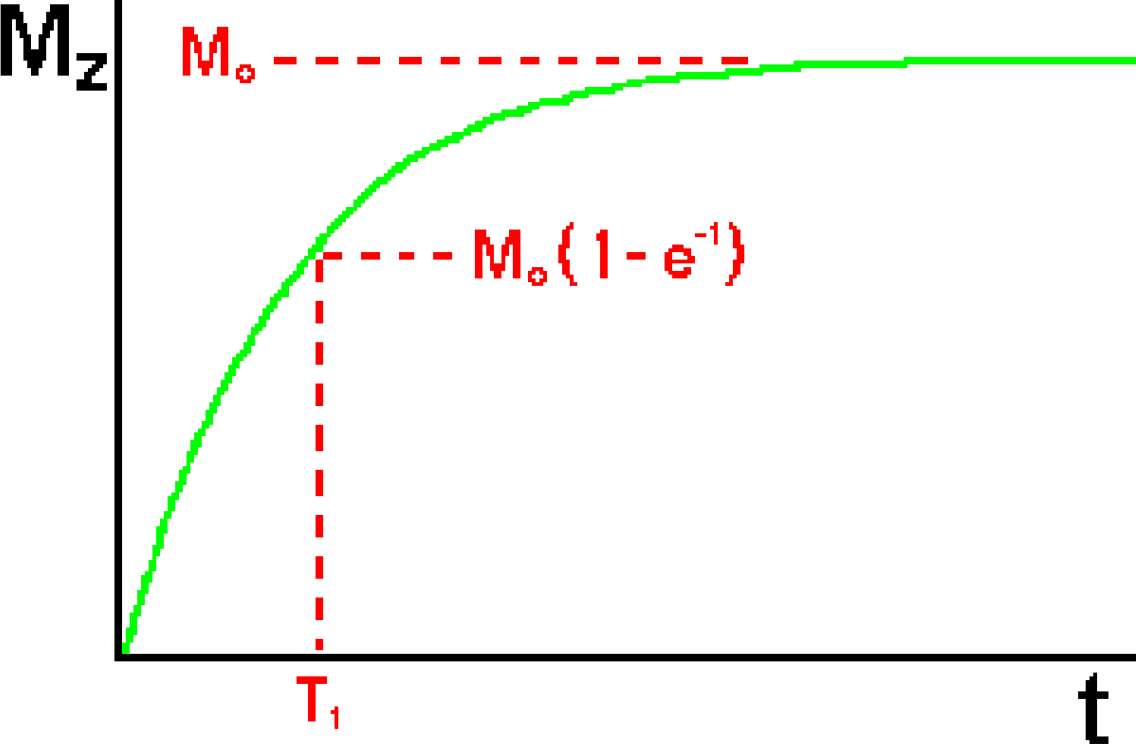
\includegraphics[width=\textwidth]{mzanstieg.png}
							\caption{}
							\label{img:anstieg}
						\end{subfigure}
						\begin{subfigure}[h]{0.48\textwidth}
							\centering
							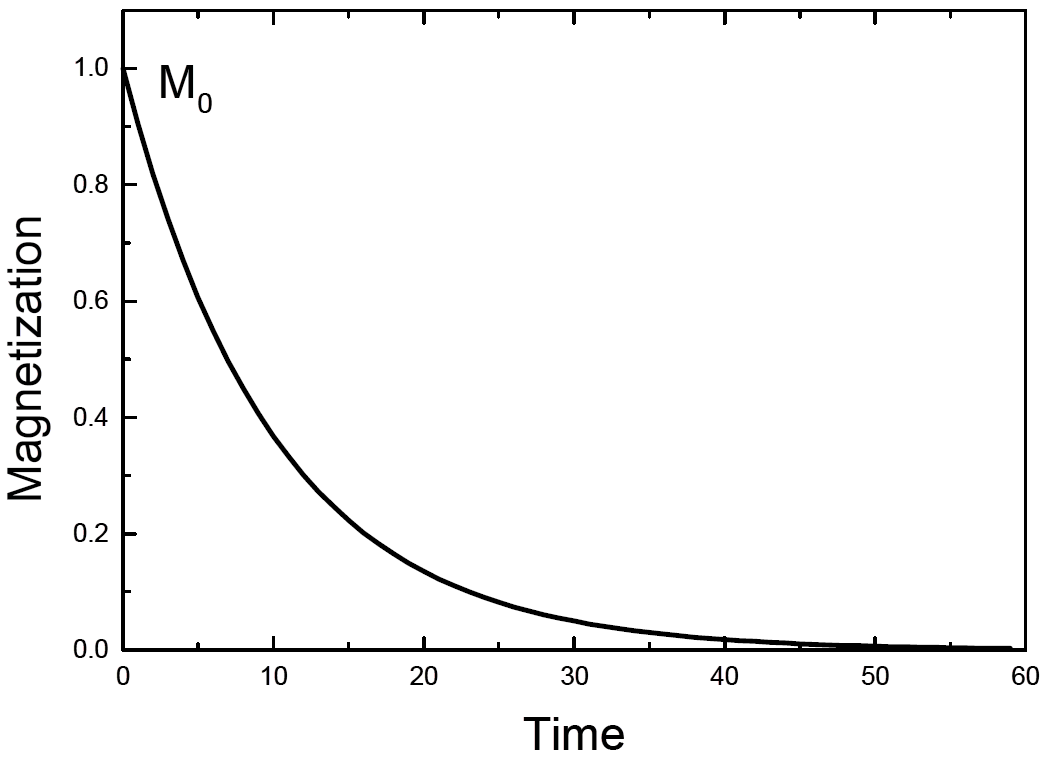
\includegraphics[width=\textwidth]{abfallm.png}
							\caption{}
							\label{img:abfall}
						\end{subfigure}
						\caption{Verlauf der Magnetisierung bei Einschalten  in z-Richtung (\autoref{img:anstieg}) und nach Ausschalten (\autoref{img:abfall}) eines externen Magnetfeldes; beliebige Probe. \cite{TeachSpinNMR}}
					\end{figure}

		\subsection{Messmethoden}\label{subsec:meth}

			Im Allgemeinen verwendet man 2 Verfahren, um die materialspezifischen Größen $T\ix{1}$ und $T\ix{2}$ zu bestimmen. Insbesondere sind diese Eigenschaften/daraus folgende Charakteristika zentraler Punkt der vielen Anwendungsbeispiele der Kernspinresonanz.
			\paragraph{Inversion-Recovery-Verfahren}
				Zuerst wird über einen zirkular polarisierten Magnetfeld-Puls der Frequenz $\omega\ix{0}$ die in +z-Richtung orientierte Magnetisierung umgedreht. Am Ende der Puls-Dauer steht diese somit in -z-Richtung; man bezeichnet eine solche Manipulation demnach als $\unit[180]{\degree}$-Puls. Nach einer pulsfreien Zeit $\tau$ gibt man einen $\unit[90]{\degree}$-Signal ein. Die Spins, welche sich während der Wartezeit $\tau$ schon wieder in +z-Richtung umorientiert hatten, erzeugen nun eine endliche Magnetisierung in der xy-Ebene. Man "`checkt"' quasi, welche z-Magnetisierung nach $\tau$ vorliegt. Variiert man diese Wartezeit, so kann man die gesamte Spin-Korrelation und dessen Relaxation vermessen. Zu erwarten ist der Verlauf von \autoref{eq:magnetumkl} bzw. \autoref{img:abfall}, wobei man nach der Größe $T\ix{1}$ sucht.
			\paragraph{Spin-Echo-Verfahren}
				Auf Grund von thermischen Prozessen und Inhomogenitäten in externen Feldern und der Substanz selbst '\tilt{klappen}' nicht alle Spins gleichermaßen hin und her, weswegen sie nicht als in-Phase während einer Messung angenommen werden können. Die \autoref{img:umklappen} macht den Sachverhalt der Spin-Echo-Methode sehr anschaulich.\\
				Nach einem $\unit[90]{\degree}$-Puls (oder auch $\pi/2$) liegt der Magnetisierungs-Vektor in der xy-Ebene. Die auseinander gedrifteten Spins werden anschließend nach einer Wartezeit $\tau$ mit einem $\unit[180]{\degree}$-Signal ($pi$) umgedreht und wieder \tilt{fokussiert}. Die Magnetisierung steigt erneut an, wenn sich die gesammelten Spins in Ausgangsrichtung des stationären Magnetfeldes befinden. Dieses \tilt{Echo} der Magnetisierung ist nach der Spin-Spin-Relaxationszeit $2\tau=T\ix{2}$ zu beobachten.\\
				Sind die Einflüssen von Störungen groß bzw. schnell gegen die Spin-Spin-Relaxation, so kommt es zu keinem kollektiven Echo. Die Zeit $T\ix{2}$ kann nicht angemessen bestimmt werden. Die Verfahren nach \tilt{Carr-Purcell} und \tilt{Meibomm-Gill} umgehen diese Problematik, indem beide eine Sequenz von $\unit[180]{\degree}$-Pulsen verwenden (siehe \autoref{sec:auswert}).

					\begin{figure}[h]
						\centering
						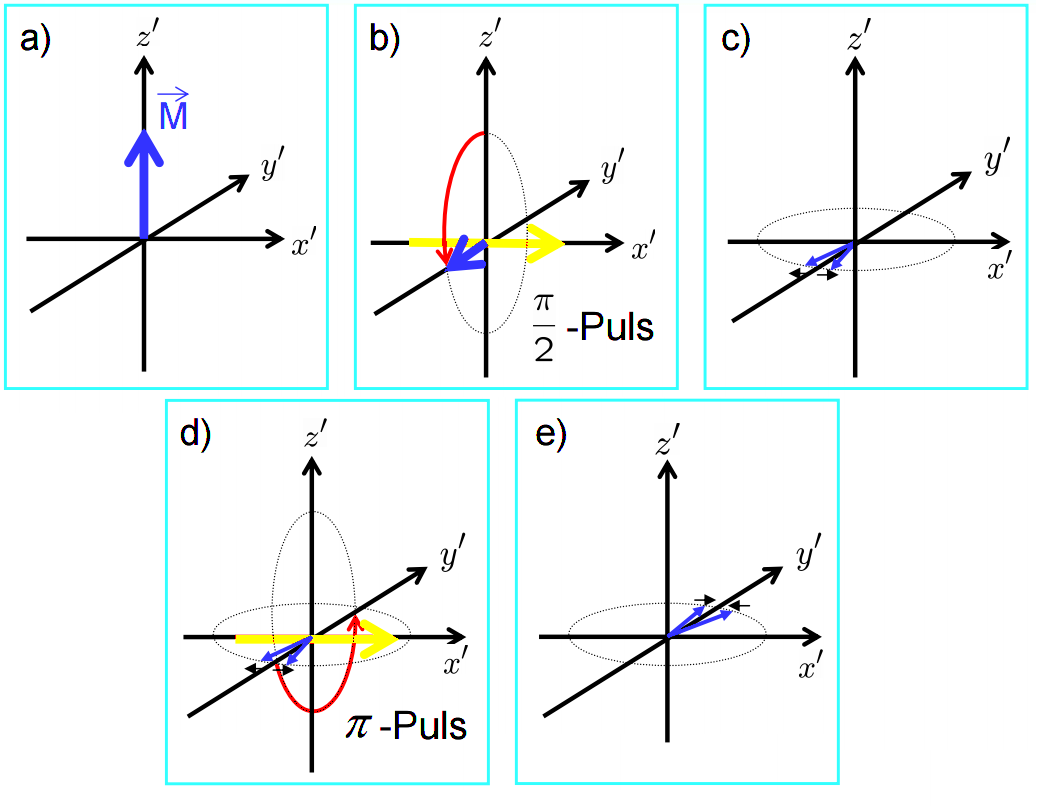
\includegraphics[width=0.8\textwidth]{umklappen.png}
						\caption{Verlauf der Spin-Echo-Methode . \fett{a):} Ausgangssituation. \fett{b):} ein $\unit[90]{\degree}$-Puls bringt die Spins in die xy-Ebene. Eine Störung (gelb) verursacht das aus-der-Phase-Laufen in \fett{c)}. Die Nettomagnetisierung verschmiert. \fett{d):} ein $\unit[180]{\degree}$-Signal führt die präzidierenden Spin-Anteile zusammen. Nach der Zeit $2\tau$ beobachtet man das Spin-Spin-Relaxations-Echo.\cite{UAchenNMR}}
						\label{img:umklappen}
					\end{figure}

	\clearpage
	\section{Durchführung}

		Der Versuchsaufbau mit \fett{TeachSpin}-Magnetfeldgenerator, Oszilloskop, Feldgradient-Controller und Steuereinheit des Generators zeigt \autoref{img:aufbau}. Die Inbetriebnahme und Kalibrierung des Experiments erfolgte nach \cite{EMAUGreifswaldNMR}. Dabei galt es, die Resonanzfrequenz des Wasserstoffatomkerns (Protonen) möglichst genau einzustellen. Die Messmethode selbst geht hauptsächlich auf die Messung eines, durch die veränderliche Magnetisierung der Probe hervorgerufenen Induktionsstromes zurück. \\
		Anschließend wurden mit Hilfe des Oszilloskops für die drei Proben Wasser, Alkohol und Feinmechanik-Öl anhand des \tilt{free induction decay} die Spin-Spin- und Spin-Gitter-Relaxationszeiten abgeschätzt. Über die Variation der Puls-Länge wird hierbei ein maximales Signal gesucht. Die ermittelten Größen benutzt man in den Verfahren aus \autoref{subsec:meth} für alle Substanzen, woraus in \autoref{sec:auswert} die Materialgrößen $T\ix{1}$ und $T\ix{2}$ bestimmt werden können.

			\begin{figure}[h]
				\centering
				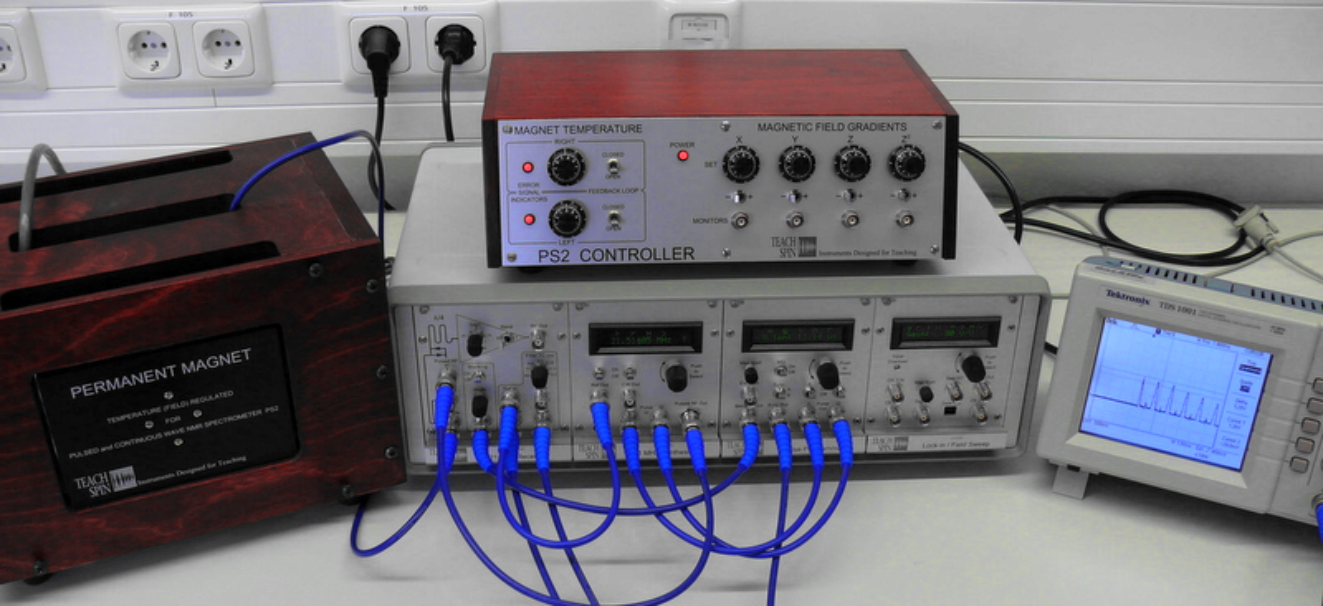
\includegraphics[width=\textwidth]{aufbau.png}
				\caption{Versuchsaufbau nach \cite{UAchenNMR} bzw. \cite{EMAUGreifswaldNMR} mit Magnetfeldgenerator, Oszilloskop, Feldgradient-Controller und Steuereinheit.}
			\end{figure}

	\clearpage
	\section{Auswertung}\label{sec:auswert}

	\clearpage
	\section{Anhang}

		\bibliography{all.bib}
		\bibliographystyle{unsrt}

\end{document}